% porque
\chapter{Motivação}
\label{chap:motivacao}

\section{Introdução}
\label{motivacao:sec:introducao}



Ao longo dos anos o crescimento da utilização de serviços informáticos, de dispositivos mais acessíveis à população mundial e uma maior cobertura de serviços de Internet
tem levado ao aumento da necessidade de serviços com uma maior escalabilidade, para garantir o acesso a mais utilizadores, com uma maior disponibilidade, 
visto que erros do sistema ou \emph{Downtime} tornam-se uma inconveniência para os utilizadores,
e distribuídos geograficamente, para garantir o acesso mais rápido ao serviço.

Também o aumento do número de núcleos nos processadores ou a eficiência de várias máquinas trabalharem em conjunto
tem vindo a aumentar a utilização de programas concorrentes e sistemas distribuídos.

Das várias vantagens no uso de sistemas distribuídos, as que mais se destacam são as seguintes.
\begin{description}
    \item [Escalabilidade Horizontal] - Os sistemas distribuídos permitem que se aumente a capacidade de processamento
	e armazenamento ao introduzir máquinas no sistema ao invés de melhorar uma única máquina.
	
    \item [Maior tolerância a erros] - Quando o processamento está distribuído por vários nós, a falha de um único nó não levará a que a todo o sistema falhe.

    \item [Mais eficientes] - O uso de algoritmos distribuídos permite um maior número de máquinas em execução concorrente, e consequentemente, a divisão do trabalho pelas várias máquinas.
	Também é possível a distribuição da localização física das máquinas, o que permite conexões de maior velocidade em outros locais no mundo.

\end{description}

No entanto, os sistemas distribuídos, que inerentemente são concorrentes,
têm uma complexidade maior no desenvolvimento em comparação com sistemas/programas sequenciais/de um único processo.
A falta de um relógio central,
a possibilidade de vários processos necessitarem de aceder ao mesmo recurso ao mesmo tempo,
ordem indeterminada de quais quer eventos,
a necessidade de se usar uma rede para comunicar informação entre os nós e dificuldade de controlar 
os vários sistemas independentes pertencentes ao sistema distribuídos são alguns dos fatores para esta complexidade.

Um dos tópicos relacionado com o protocolo estudado é o acesso ao mesmo recurso por vários processos.

Por exemplo, várias máquinas numa rede têm a possibilidade de aceder a um ficheiro, tanto para fazer uma leitura como uma escrita.
Duas máquinas (ou processos) pretendem fazer alterações num ficheiro na rede, ambas começam por fazer uma leitura do ficheiro, e após essa leitura, uma das máquinas escreve as alterações, e logo de seguida a outra máquina escreve as alterações. A falha nesta ocorrência foi que a última máquina a escrever sobrescreveu totalmente as a alterações da primeira, visto que ambas leram o mesmo estado do ficheiro mas a uma das máquinas escreveu após a escrita da outra.

Este tipo de ocorrências são denominadas de falha de Condição de Corrida ou \emph{Race Condition},
que podem levar a estados inesperados de qualquer elemento se possa ser alterado (como ficheiros, estruturas de dados, etc),
que por último podem levar a grandes catástrofes.

% Melhorar
Um exemplo catastrófico foi o ``Apagão de 2003'' \cite{blackout} que afetou os Estados Unidos da América e Canada. 

Após falharem 3 linhas de eletricidade, foram enviados 3 pedidos ao ``mesmo tempo'', que provocou uma \emph{Race Condition} na escrita de nova informação num servidor central, deixando assim o servidor num estado corrupto/errado.
Essa corrupção levou a que o sistema de alarme entrasse em Ciclo Infinito, fazendo com que não fosse possível receber novos avisos de outras linhas.

No protocolo estudado, estes problemas são evitados através da criação de uma fila, esta distribuída, que ordena/sincroniza o acesso ao objeto por parte dos vários nós do sistema.
A formação desta fila é descrita com maior pormenor na secção \ref{motivacao:sec:descricao_protocolo}. 

\section{Descrição do Protocolo}
\label{motivacao:sec:descricao_protocolo}

Nesta secção será descrito o funcionamento e estrutura do \textit{Arrow Distributed Directory Protocol} (\emph{Arrow}) \cite{Arrow}. 

Este sistema consiste numa rede, que permite o envio assíncrono de mensagens (ou a comunicação) entre os nós, e um diretório, que permite localizar um objeto na rede e garantir o acesso exclusivo a este. 

O diretório pode ser considerado como um grafo, em que os nós do grafo são os vários elementos que pertencem ao sistema (por exemplo, várias instâncias de um programa ou máquinas na rede) e as arestas são as várias ligações no diretório entre os vários Nós.


Consideramos que o objeto é ``móvel'', no entanto esta é uma abstração do \textbf{acesso} ao objeto, e este acesso tem a possibilidade de se movimentar na rede entre os nós.

O objeto pode ser um processo, um ficheiro ou qualquer outra estrutura de dados.

Cada nó tem uma só ligação, deste para outro nó, no entanto podem existir vários nós com ligação a um único nó.

Quando um nó pretende aceder ao objeto, este envia um pedido de acesso pela sua ligação. 



Consideremos que a noção que o diretório é uma árvore de extensão mínima, e consideremos que o acesso ao objeto (ou o nó que o detém) está localizado na raiz da árvore e todas as ligações apontam em direção à raiz.

Quando é realizado um pedido, este irá chegar à raiz, pois todas as ligações apontam para esta. No final da circulação do pedido, todas as ligações por onde passou o pedido estão invertidas, para que estas passem a apontar para o nó que fez o pedido.

Caso um nó receba um pedido de acesso,a ligação deste passa a apontar para o nó vizinho que lhe fez chegar o pedido, ou seja, por onde passa o pedido há uma inversão do sentido da ligação.



\subsection*{Exemplo da organização das ligações}

Vejamos o seguinte exemplo da rede \ref{motivacao:img:estado_inicial}, em que o (acesso ao) objeto se encontra atualmente no nó \textbf{H}.


\begin{figure}[!htb]
\centering
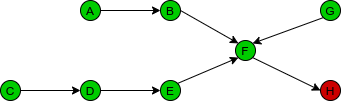
\includegraphics[width=250pt]{um_pedido_1.png}
\caption{Estado inicial do diretório}
\label{motivacao:img:estado_inicial}
\end{figure}

O nó \textbf{A} pretende obter o acesso ao objeto, e para tal envia um pedido através da sua ligação (para o nó \textbf{B}).
O pedido passará pelos nós \textbf{B}, \textbf{F} e \textbf{H}, por esta ordem.

Vejamos o estado após o pedido chegar ao nó \textbf{F}, como demonstrado na imagem \ref{motivacao:img:apos_chegar_f}:

\begin{figure}[!htb]
\centering
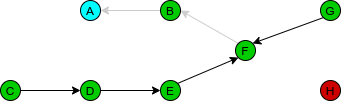
\includegraphics[width=250pt]{um_pedido_2.png}
\caption{Estado do diretório após o pedido chegar ao nó \textbf{F}}
Note que as ligações por onde o pedido do nó \textbf{A} passou inverteram-se.
\label{motivacao:img:apos_chegar_f}
\end{figure}


Quando o nó \textbf{A} faz o pedido e este chega ao \textbf{H} este passa a ser a raiz da árvore,
e os seguintes pedidos serão direcionados até ao \textbf{A}.\\



Vejamos agora outro exemplo \ref{motivacao:img:apos_chegar_f_etiquetas},
em que exploramos o caso de existirem mais do que uma mensagem a circular no diretório:

Consideremos que cada passo é uma transmissão de pedidos entre nós, e que os passos que cada pedido executa são sincronizados com os restantes,
algo que não é garantido na rede, mas que temos em conta para se demonstrar com maior simplicidade este processo.

Consideremos o mesmo estado anteriormente referido,
o estado do diretório após o pedido do nó \textbf{A} chegar ao nó \textbf{F}, 
e que ao mesmo tempo o nó \textbf{D} pretende obter o acesso,
que para tal este enviou um pedido de acesso que atualmente se encontra no nó \textbf{E}.


\begin{figure}[!htb]
\centering
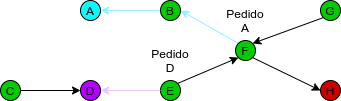
\includegraphics[width=250pt]{dois_pedidos_1.png}
\caption{Estado do diretório após o pedido do nó \textbf{A} chegar ao nó \textbf{F} e o pedido do nó \textbf{D} chegar ao nó \textbf{E}. 
As etiquetas com ``Pedido'' indicam onde o pedido de cada nó se encontra no atual estado.}
\label{motivacao:img:apos_chegar_f_etiquetas}
\end{figure}

Como o nó \textbf{F} aponta/está ligado ao nó \textbf{B}, o pedido do nó \textbf{D} será então transmitido para este ao invés do \textbf{H}.
Vejamos o passo seguinte deste estado na imagem \ref{motivacao:img:d_chega_f}:


\begin{figure}[!htb]
\centering
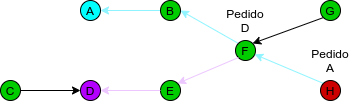
\includegraphics[width=250pt]{dois_pedidos_2.png}
\caption{Estado do diretório após o pedido do nó \textbf{D} chegar ao nó \textbf{F}}
\label{motivacao:img:d_chega_f}
\end{figure}

\textbf{Nota:} Caso os dois pedidos chegassem ao nó \textbf{F}, e que nenhum dos dois ainda não foi tratado, os pedidos terão de ser tratados de cada vez. Se o pedido do nó \textbf{A} fosse o primeiro a ser processado, este seria transmitido para o \textbf{H} e o pedido do \textbf{D} continuava a circulação em direção ao \textbf{A} e vice-versa. \\

No passo seguinte \ref{motivacao:img:d_chega_b}, o pedido do \textbf{D} encontra-se no nó \textbf{B}:


\begin{figure}[!htb]
\centering
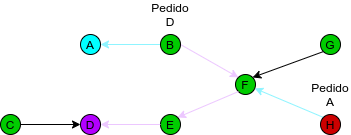
\includegraphics[width=250pt]{dois_pedidos_3.png}
\caption{Estado do diretório após o pedido do nó \textbf{D} chegar ao nó \textbf{B}}
\label{motivacao:img:d_chega_b}
\end{figure}

%%%%%%%%%%%%%%%%%%%%%%%%%%%%%%%

Numa vista global sobre a rede, quando um nó realiza um pedido, as ligações dos nós por onde esse pedido passou passam a indicar onde é que futuramente estará o objeto, ou seja, na direção do nó que fez o pedido e que espera pelo acesso ao objeto.
Qualquer outra ``sobreposição'' das alterações nas ligações fará com que as ligações apontem em direção dos nós que realizaram os pedidos que passaram por essas ligações, isto é, independentemente da quantidade de pedidos a circular na rede, se seguirmos as direções das ligações em qualquer estado da rede estas apontam sempre para um nó que detém ou espera pelo acesso ao objeto.

Esta inversão das ligações permite que, o nó apenas detendo uma ligação, faça chegar o seu pedido ao nó que detém o objeto ou a um nó que deterá o objeto mas que espera por ele. \\




Caso um nó que espera pelo objeto, quer porque o seu pedido ainda está em circulação na rede ou o nó detentor do objeto ainda não o cedeu, receba um pedido de acesso de outro nó, então este armazena uma ligação com o nó que realizou o pedido.

Quando o nó que detém o objeto, recebe um pedido ou tem em espera um outro nó, o objeto é cedido através de uma ligação direta entre dois nós, evitando a passagem do objeto pelo diretório.


\subsection*{Exemplo da formação de uma fila de espera}

Continuando o exemplo anterior. Vejamos um passo seguinte, em que o pedido do nó \textbf{D} chega ao nó \textbf{A}, o nó \textbf{H} ainda não cedeu o acesso ao nó \textbf{A}, e o nó \textbf{C} decidiu realizar um pedido que atualmente se encontra no nó \textbf{D}, que também está à espera do acesso ao objeto. Vejamos a imagem \ref{motivacao:img:3_pedidos}.

\begin{figure}[!htb]
\centering
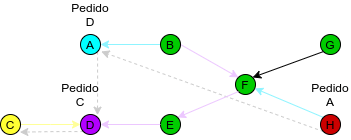
\includegraphics[width=250pt]{fila.png}
\caption{Estado do diretório com 3 pedidos em circulação.}
\label{motivacao:img:3_pedidos}
\textbf{Nota:} As ligações a tracejado representam as ligações entre os nós fora do diretório, usadas para a transmissão do acesso ao objeto.
\end{figure}


Temos assim os seguintes nós à espera:
\begin{enumerate}
    \item O nó \textbf{A} espera pelo nó \textbf{H}.
    \item O nó \textbf{D} espera pelo nó \textbf{A}.
    \item O nó \textbf{C} espera pelo nó \textbf{D}.
\end{enumerate}
Ou seja, a ordem de chegada e fila do acesso de pedidos será a \textbf{A},\textbf{D},\textbf{C}. \\


 

\noindent A particularidade deste protocolo deve-se à mudança tanto da localização do objeto como a sua origem, pois esta muda-se para o nó que tem o acesso ao objeto, e não há um único nó que detém a localização atual do objeto, mas a disposição de todas as ligações permite a localização do objeto por todos os nós.

O facto da ``Casa'' do objeto estar em constante alteração garante que apenas um nó detenha o acesso ao objeto (acesso exclusivo), e que o único detentor do objeto se torne num foco, isto é, que nenhum nó receba demasiados pedidos em relação a outros nós, provocado um engarrafamento/\emph{bottleneck} no acesso ao objeto.

% notas paper
% explicar o nome
% explicar que ao seguirmos as setas chegamos sempre ao objeto ou alguém que terá acesso ao mesmo
% explicar o que é um diretório
% dar uma vista global sobre
% - Objeto Movível
% O objeto move-se pelo diretório dependendo se houve pedidos por parte de Nodes

\subsection*{Estruturas de Dados}
Neste protocolo existem duas estruturas distribuídas, em que cada uma é formada por um tipo de ligação entre os nós.

\begin{description} 
    \item [Grafo] os vértices são todos os nós do sistema, e as arestas são as ligações entre os nós utilizadas no envio de pedidos de acesso.
    \item [Fila] os vértices são todos os nós do sistema que esperam pelo acesso ao objeto  e as arestas são as ligações entre os nós mas exterior ao diretório, pois neste circula o acesso ao objeto.
\end{description}

\section{Trabalhos Relacionados}
\label{motivacao:sec:trabalhos_relacionados}
%Ivy e Arvy

% TODO: Explicar quais é que são os benefícios de usar cada um
Existem dois algoritmos cujo o seu funcionamento é semelhante com o \acs*{ADDP}.
Estes são o \emph{Ivy} \cite{Ivy} e o \emph{Arvy} \cite{Arvy}, este último sendo uma generalização de ambos o \emph{Ivy} e o algoritmo estudado (\acs{ADDP}).
Este três algoritmos (ou classe de algoritmos) garantem o acesso exclusivo ao objeto (ou o acesso a este) fazendo uso de mecanismos de mudança de ligações.
O \emph{Ivy} apresenta um funcionamento muito similar ao \emph{Arrow} (\acs*{ADDP}),
em que o objeto (ou o acesso a este) varia de localização,
mas destaca-se do \emph{Arrow} na formação das ligações, que,
ao invés de as ligações por onde o pedido passa se inverterem,
os \emph{Nodes} que recebem os pedidos passam a estar ligados ao \emph{Node} que realizou o pedido.

Como referido anteriormente, o \emph{Arvy} é uma generalização de ambos.
Neste algoritmo, quando um \emph{Node} recebe um pedido este pode ligar-se a qualquer \emph{Node} por onde atravessou o pedido.


Quanto a implementações, existem três relacionadas com a desenvolvida neste projeto. 
Estas são, o \emph{Aleph Toolkit}\cite{aleph}, a qual é a única implementação conhecida do \acs*{ADDP}, mas esta é muito diferente da obtida no decorrer deste projeto, 
a implementação do \emph{Arvy} \cite{ArvyImpl}, a qual já foi referida, 
e uma implementação do \emph{Bully Algorithm} \cite{bully}, que inspirou o uso de uma Página \emph{Web}, esta que comunica com um nó de visualização para a visualização do sistema distribuído, e 
também inspirou o uso do \emph{Docker} para o \emph{Deploy}/execução do sistema, no entanto este tópico será exposto num capítulo seguinte (Capítulo \ref{chap:engenharia}).



\section{Conclusões}
\label{motivacao:sec:conclusao}

%Mudar a palavra esclarecido
Neste capítulo foi descrito o aumento da necessidade de sistemas e algoritmos distribuídos bem construídos, tal como a complexidade de implementação dos mesmos.

No contexto deste projeto, das falhas que ocorrem somente em sistemas concorrentes (e por sua vez, distribuídos), a que se pretende evitar (principalmente)
é a Condição de Corrida/\emph{Race Condition},
pois este tipo de falhas provoca resultados/estados inesperados de sistemas e informação, por vezes provocando catástrofes ou grandes problemas.

O protocolo em questão evita este tipo de falhas ao garantir que, a qualquer momento, apenas um elemento detém o (acesso ao) objeto.
Na descrição desenvolvida sobre este algoritmo há uma maior ênfase na mudança das ligações entre os nós e o que esta mudança provoca no sistema numa vista global e a mudança da origem do objeto,
pois este é o mecanismo que evita o acesso concorrente ao objeto, que, após um primeiro pedido chegar ao atual detentor do objeto, o detentor cederá o objeto ao autor do pedido,
e os subsequente pedidos de acesso serão redirecionados em direção a um futuro detentor.

Foram também referidos dois trabalhos relacionados com o \acs*{ADDP}, os quais diferem principalmente na formação das novas ligações após a receção de pedidos de acesso e três implementações
relacionadas à implementação realizada neste projeto.

